\documentclass{standalone}
\usepackage{tikz}
%------------tikz Setup------------

\tikzstyle{ball} = [circle,shading=ball, ball color=black,
    minimum size=1mm,inner sep=1.3pt]
\tikzstyle{miniball} = [circle,shading=ball, ball color=black,
    minimum size=1mm,inner sep=0.5pt]
\tikzstyle{mminiball} = [circle,shading=ball, ball color=black,
    minimum size=0.6mm,inner sep=0.1pt]
\usetikzlibrary{arrows.meta}
\usetikzlibrary{angles, quotes}
\tikzset{>={Latex[length=2mm,width=1.5mm]}}
\tikzset{->-/.style={decoration={markings, mark=at position #1 with
  {\arrow{>}}},postaction={decorate}}}
\usetikzlibrary{decorations.pathmorphing}
\usetikzlibrary{decorations.pathreplacing}
\usetikzlibrary{arrows.meta,calc}
\usetikzlibrary{bending}
\usetikzlibrary{decorations.markings,shapes.geometric}
\tikzset{->-/.style={decoration={markings, mark=at position #1 with
  {\arrow{>}}},postaction={decorate}}}
\tikzset{-|-/.style={decoration={markings, mark=at position #1 with
  {\arrow{stealth}}},postaction={decorate}}}
\tikzset{movearrow/.style 2 args ={
        decoration={markings,
    mark= at position {#1} with {\arrow{#2}} ,
        },
        postaction={decorate}
    }
}


\begin{document}
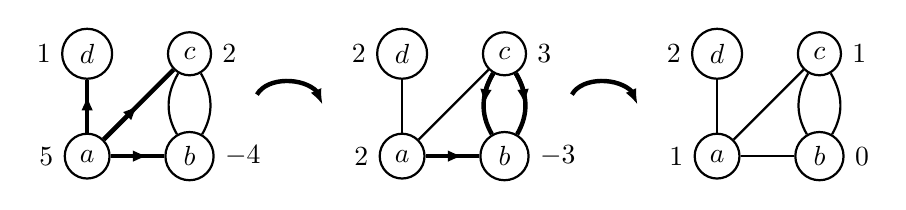
\begin{tikzpicture}[thick,main/.style = {draw, circle}]
\begin{scope}[scale=1.3]
    \node[main,label={left:$5$}] (1) at (0,0) {$a$}; 
    \node[main,label={right:$-4$}] (2) at (1,0) {$b$}; 
    \node[main,label={right:$2$}] (3) at (1,1) {$c$};
    \node[main,label={left:$1$}] (4) at (0,1) {$d$};
    \draw[ultra thick] (1) to (2);
    \draw[thick] (2) to [out=60,in=300,looseness=1] (3);
    \draw[thick] (2) to [out=120,in=240,looseness=1] (3);
    \draw[ultra thick] (3) to (1);
    \draw[ultra thick] (1) to (4);
    \draw[ultra thick,->] (1) to (0, 0.6);
    \draw[ultra thick,->] (1) to (0.6, 0);
    \draw[ultra thick,->] (1) to (0.5, 0.5);
    \node (a) at (1.6, 0.5) {};
    \node (b) at (2.3, 0.4) {};
    \draw[ultra thick,->] (a) to [out=60,in=90] (b);
\end{scope}
\begin{scope}[xshift=4cm,scale=1.3]
    \node[main,label={left:$2$}] (1) at (0,0) {$a$}; 
    \node[main,label={right:$-3$}] (2) at (1,0) {$b$}; 
    \node[main,label={right:$3$}] (3) at (1,1) {$c$};
    \node[main,label={left:$2$}] (4) at (0,1) {$d$};
    \draw[ultra thick] (1) to (2);
    \draw[ultra thick] (2) to [out=60,in=300,looseness=1] (3);
    \draw[ultra thick] (2) to [out=120,in=240,looseness=1] (3);
    \draw[thick] (3) to (1);
    \draw[thick] (1) to (4);
    \draw[ultra thick,->] (1) to (0.6, 0);
    \draw[ultra thick,->] (3) to [out=300,in=90,looseness=1] (1.2,0.5);
    \draw[ultra thick,->] (3) to [out=240,in=90,looseness=1] (0.8,0.5);
    \node (a) at (1.6, 0.5) {};
    \node (b) at (2.3, 0.4) {};
    \draw[ultra thick,->] (a) to [out=60,in=90] (b);
\end{scope}
\begin{scope}[xshift=8cm,scale=1.3]
    \node[main,label={left:$1$}] (1) at (0,0) {$a$}; 
    \node[main,label={right:$0$}] (2) at (1,0) {$b$}; 
    \node[main,label={right:$1$}] (3) at (1,1) {$c$};
    \node[main,label={left:$2$}] (4) at (0,1) {$d$};
    \draw[thick] (1) to (2);
    \draw[thick] (2) to [out=60,in=300,looseness=1] (3);
    \draw[thick] (2) to [out=120,in=240,looseness=1] (3);
    \draw[thick] (3) to (1);
    \draw[thick] (1) to (4);
\end{scope}
\end{tikzpicture}
\end{document}